\documentclass{article}
\usepackage{a4wide}
\usepackage{graphicx}
\usepackage{amsmath, amsthm, amssymb}

\usepackage[utf8]{inputenc}
\usepackage{ngerman}
\usepackage{url}
\usepackage[ruled,vlined]{algorithm2e}
\usepackage[]{hyperref}
\usepackage{listings}
\usepackage{dsfont}

\newtheorem{thm}{Theorem}[section]
\newtheorem{cor}[thm]{Korollar}
\newtheorem{lem}[thm]{Lemma}
\newtheorem{defi}[thm]{Definition}
\newtheorem{definition}{Definition}
\newcounter{Chapcounter}
\newcommand\showmycounter{\addtocounter{Chapcounter}{1}\themycounter}
\newcommand{\chapter}[1] 
{ {\centering          
  \addtocounter{Chapcounter}{1} \Large \underline{\textbf{ \color{blue} Chapter \theChapcounter: ~#1}} }   
  \addcontentsline{toc}{section}{ \color{blue} Chapter:~\theChapcounter~~ #1}    
}
\hypersetup{colorlinks=true}
\hypersetup{linkcolor=black}
\usepackage{listings}
\lstdefinelanguage{Pseudo}{
  morekeywords={forall,if,then,else,return,while,do,for,DFS},
  sensitive=false,
  morecomment=[l]{//},
  morestring=[b]"
}



\setcounter{tocdepth}{4}

\begin{document}
\title{Programmierparadigmen}
\date{Sommersemester 2026}
\author{Universität Stuttgart}
\maketitle
\tableofcontents
\newpage

\section{Preface}
The idea of these notes is to be written in english, but it is possible that some words appear in German/Spanish, given that english is not my frst language.

These notes contain all topics I valued as important for the exam, but some stuff that may have been trivial for me may not appear in the notes. So if anybody is using my notes to 
prepare for the exam, please be wary of this.
\section{Alias list}
\begin{itemize}
  \item PL: Programming Language
\end{itemize}

\section{Basics/ Organizational}
This lecture is about concepts for each language, not a deep dive on a specific language, but an understanding of tradeoffs and features

\begin{itemize}
  \item Final exam in english (can be answered in german too), but lectures in german
  \item 6 excersises, 14 days to solve
  \item Quizzes during each lecture (give bonus points for schein)
  \item To go to the exam there are 6 excersises 100 points each
  \begin{itemize}
    \item 30 points in 5 excersises
    \item 360 total points
  \end{itemize}
  \item All help allowed for the exam except electronic. Not sure if printed stuff is allowed.
\end{itemize}

\section{History}
\subsection{Bits}
First computers were programmed in machine language, as a sequence of bits. Machine time
was more valuable than developer time.

\subsection{Assembly}
Human-readable abbreviations for machine language instructions. Each new machine had different assembly language
but it was less error prone than raw bits.

The developer is forced o think in terms of very low level operations,
directly interacting with the hardware

\subsection{High level languages}
First high level languages were Fortran, Lisp\dots More logical and mathematical abstractions.

\subsection{Today}
1000s of languages, each with their own toolkit and feature set

\section{Spectrum of PL}
\subsection{PL types}
\begin{itemize}
  \item Declarative: Haskell, SQL
  \item Impertative: Java, C
  \item Logical (more mathematical): Prolog 
\end{itemize}

\subsection{Execution types}
\begin{itemize}
  \item Interpretation (basic Lisp interpreter)
  \item Compilation (C)
  \item Mix of both (Java has VM with just-in-time compilation, Python is compiled to bytecode then interpreted)
\end{itemize}


\section{Syntax vs.\ Semantics}
This describes the difference between the structure of code and its meaning.

\begin{itemize}
  \item \textbf{Syntax}: how code is written (structure, rules)
  \item \textbf{Semantics}: what the code actually means / does
\end{itemize}

\subsection{Syntax in Different Programming Languages}
Most programming languages have different syntax but similar semantics.

\textbf{Example:}

Java:
\begin{lstlisting}[language=Java]
if (foo > 100) {
  System.out.println("Hello World!");
}
\end{lstlisting}

Bash:
\begin{lstlisting}[language=Bash]
if [ $foo -gt 100 ]
then
  echo "Hello World!"
fi
\end{lstlisting}

\medskip
However, sometimes languages share similar syntax but differ in semantics.

\textbf{Example: Java vs.\ JavaScript}
\begin{lstlisting}
if ("abc" != 5) {
  ...
}
\end{lstlisting}

\begin{itemize}
  \item In Java: type error at compile time
  \item In JavaScript: implicit type conversion is performed (no error)
\end{itemize}

\subsubsection{Four Concepts to Specify Syntax}
\begin{itemize}
  \item Concatenation
  \item Alternation / choice
  \item Repetition (Kleene closure)
  \item Recursion
\end{itemize}

These concepts form the basis of regular expressions and extend to context-free grammars.

\section{Syntax}

\subsection{Tokens}
Tokens are the basic building blocks of a programming language.

\paragraph{Example (C)}
\begin{itemize}
  \item Keywords: \texttt{double}, \texttt{if}, \texttt{return}, \texttt{struct}
  \item Punctuators: \texttt{,}
  \item Literals: \texttt{'x'}
  \item Identifiers: \texttt{printf}
\end{itemize}

Tokens are typically specified using regular expressions (see Theo).

\subsubsection{Identifiers in Different Languages}
\begin{itemize}
  \item Some languages (e.g.\ Ada, Pascal) are case-insensitive
  \item Letters and digits are almost always allowed
  \item Underscores are usually allowed
\end{itemize}

\paragraph{Naming Conventions}
\begin{itemize}
  \item Java:
  \begin{itemize}
    \item Classes: \texttt{ClassName}
    \item Variables: \texttt{variableName}
  \end{itemize}
\end{itemize}

\subsubsection{Formatting}
Depending on the language, indentation and line breaks may or may not affect program behavior.

% --------------------------------------------------

\subsection{Context-Free Grammars (CFG)}

\textbf{Question:} Are regular expressions sufficient?

\textbf{Answer:} \textbf{No.}

\paragraph{Example: Arithmetic expressions}
\[
5 + 7
\]
\[
(5 + 7) + 6
\]
\[
((5 + 7) + 6) - 23
\]

These expressions grow in nested structures (``boxes''), which require recursion.  
Regular expressions do not support recursion.

\paragraph{Conclusion}
CFG $=$ regular expressions $+$ recursion

\subsubsection{Definition}
\[
G = (N, T, R, s)
\]
\begin{itemize}
  \item $N$: non-terminals (finite set)
  \item $T$: terminals (finite set)
  \item $R$: production rules, $N \to (N \cup T)^*$
  \item $s$: start symbol
\end{itemize}

\textit{(Details covered more deeply in Theo 1.)}

\subsubsection{Extensions of CFG Syntax}
\begin{itemize}
  \item Kleene star ($*$)
  \item Kleene plus ($+$)
  \item Alternation ($|$)
\end{itemize}

\subsubsection{Derivations}
A derivation is the process of generating a string from a grammar by repeatedly applying production rules until only terminals remain.

\subsubsection{Parse Trees}
A tree representation of a derivation:
\begin{itemize}
  \item Root: start symbol
  \item Inner nodes: non-terminals
  \item Leaves: terminals (tokens)
\end{itemize}

\paragraph{Remark}
A language can have infinitely many grammars, some of which are ambiguous (multiple derivations for the same string).  
A good grammar reflects the internal structure of the programming language.

% --------------------------------------------------

\subsection{Scanning}

Converting a sequence of characters in the source code into a sequence of tokens.  
This is done using regular expressions to specify tokens.

\subsubsection{Implementing a Scanner}
Read one character at a time. If a token is recognized, return it and continue. Otherwise, raise an error.

\subsubsection{Option 1: Ad-hoc Scanner}
\begin{itemize}
  \item Manually implemented
  \item Handles common tokens first
  \item Used in many production compilers due to compact code and efficiency
\end{itemize}

\subsubsection{Option 2: Finite Automata}
\begin{itemize}
  \item Each token is specified by a regular expression
  \item Finite automata = recognizers of regular expressions
\end{itemize}

Pipeline:
\[
\text{RegEx} \rightarrow \text{NFA} \rightarrow \text{DFA} \rightarrow \text{Minimal DFA}
\]

\paragraph{From DFA to Scanner}

\begin{itemize}
  \item \textbf{Switch-based implementation}
  \begin{lstlisting}
loop:
  switch (state) {
    case S1:
      switch (character) {
        case 'a': state = S2; break;
        default: error();
      }
  }
  \end{lstlisting}

  \item \textbf{Table-based scanner}
  
  Table represents states and transitions; can use a generic driver program.

  \begin{center}
    \begin{tabular}{|c|c|c|c|}
      \hline 
      State & 'a' & 'b' & Return \\
      \hline
      S1 & S2 & - & - \\
      \hline
    \end{tabular}
  \end{center}
\end{itemize}

\paragraph{Multiple Tokens}
So far: only one kind of token is recognized.  
Goal: recognize multiple token types.

\textbf{Idea:} Merge multiple token-level automata into a single automaton.

\paragraph{Longest Match Rule}
Example: $3.1$ vs.\ $3.1415$ → choose the longest valid token.

This requires lookahead.

% --------------------------------------------------

\subsection{Parsing}

Converting the sequence of tokens into a syntax tree.  
Specified using a CFG.

\subsubsection{Top-down Parsing}
\begin{itemize}
  \item Start from root node
  \item Expand non-terminals until reaching terminals
  \item If multiple rules apply, predict
\end{itemize}

\subsubsection{Bottom-up Parsing}
\begin{itemize}
  \item Start from input tokens
  \item Combine tokens into subtrees
  \item Build tree upwards
\end{itemize}

\subsubsection{Parser Classification}

\begin{center}
\begin{tabular}{|c|c|c|}
  \hline
   & LL(k) & LR(k) \\
  \hline
  Parse tree construction & Top-down & Bottom-up \\
  \hline
  Scanning & Left-to-right & Left-to-right \\
  \hline
  Derivation & Left-most & Right-most \\
  \hline
  Algorithm & Predictive & Shift-reduce \\
  \hline
\end{tabular}
\end{center}

% --------------------------------------------------

\subsubsection{LL(k) Parsers (Top-down)}

\textbf{L}eft-to-right scanning, \textbf{L}eft-most derivation, \textbf{k}-token lookahead

\paragraph{Approaches}
\begin{itemize}
  \item Recursive descent parser
  \item Table-driven LL parser
\end{itemize}

\paragraph{General Algorithm}
\begin{lstlisting}
Start with start symbol

Repeat until no more input:
  Given current non-terminal and next k tokens:
    choose production rule R

  For each symbol X in R:
    if X is non-terminal:
      expand X
    else if X is terminal:
      if next token matches X:
        consume token
      else:
        error
\end{lstlisting}

\paragraph{Recursive Descent Parser}
\begin{itemize}
  \item One function per non-terminal
  \item Chooses production using lookahead
  \item Calls functions recursively
  \item match(): consumes token or raises error
\end{itemize}

\subsubsection{Example: Recursive Descent Parser}

\paragraph{Grammar}
\begin{itemize}
  \item $S \to aB$
  \item $S \to bC$
  \item $B \to bbC$
  \item $C \to cc$
\end{itemize}

\paragraph{Parser}
\begin{lstlisting}
S() {
  if (inputToken == a) {
    match(a); B();
  } else if (inputToken == b) {
    match(b); C();
  } else {
    error();
  }
}

B() {
  if (inputToken == b) {
    match(b); match(b); C();
  } else {
    error();
  }
}

C() {
  if (inputToken == c) {
    match(c); match(c);
  } else {
    error();
  }
}
\end{lstlisting}

% --------------------------------------------------

\subsubsection{Generating a Top-Down Parser}

\begin{itemize}
  \item We must predict which production rule to apply
  \item This is done using \textbf{PREDICT} sets, based on FIRST and FOLLOW
\end{itemize}

\paragraph{FIRST(N)}
Set of terminals that can appear at the beginning of strings derived from $N$.

\begin{itemize}
  \item For a terminal $a$: FIRST$(a) = \{a\}$ (including $\varepsilon$, but only if it's \textbf{only} $\varepsilon$ within a single transition)
\end{itemize}

Example:
\begin{itemize}
  \item $S \to \text{simple} \mid \text{begin } S \text{ end}$
  \item FIRST$(S) = \{\text{simple}, \text{begin}\}$
\end{itemize}

\paragraph{FOLLOW(N)}
Set of terminals that can appear immediately to the right of $N$ in some sentential form. Only applicable to non-terminals

\begin{itemize}
  \item Includes the end-of-input symbol $\$$
  \item Never contains $\varepsilon$
\end{itemize}

Example:
\begin{itemize}
  \item $S \to \text{aBc}$
  \item $B \to d$
  \item FOLLOW$(S) = \{\$\}$
  \item FOLLOW$(B) = \{\text{c}\}$
\end{itemize}

\paragraph{Computing FOLLOW sets}
Apply the following rules until no changes occur:

\begin{enumerate}
  \item If $A$ is the start symbol, add $\$$ to FOLLOW$(A)$
  \item If $B \to \alpha A \beta$, add FIRST$(\beta) \setminus \{\varepsilon\}$ to FOLLOW$(A)$
  \item If $B \to \alpha A$, or $B \to \alpha A \beta$ with $\beta \Rightarrow^* \varepsilon$, add FOLLOW$(B)$ to FOLLOW$(A)$
\end{enumerate}

\begin{center} 
  Here is an example

  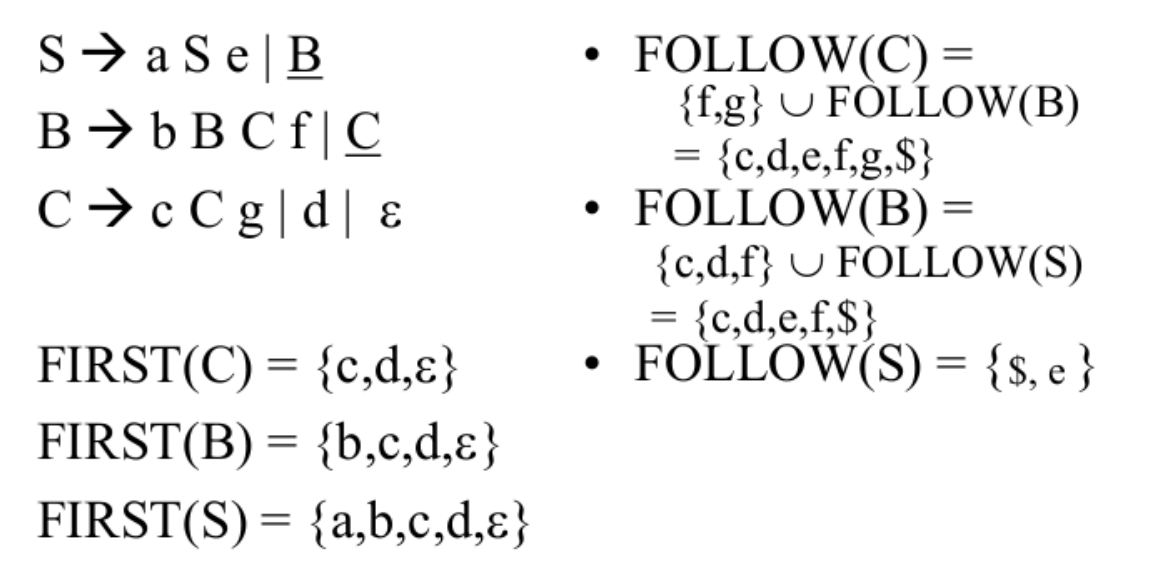
\includegraphics[scale=0.4]{assets/follow_set_computation.png}
\end{center}

\paragraph{PREDICT sets}
Determine when a production should be used in an LL(1) parser.

\begin{itemize}
  \item If the next input token is in PREDICT$(A \to \alpha)$, apply the rule $A \to \alpha$
\end{itemize}

For a production $A \to \alpha$:
\begin{itemize}
  \item If $\varepsilon \in \text{FIRST}(\alpha)$:
  \[
  \text{PREDICT}(A \to \alpha) = \big(\text{FIRST}(\alpha) \setminus \{\varepsilon\}\big) \cup \text{FOLLOW}(A)
  \]
  \item Otherwise:
  \[
  \text{PREDICT}(A \to \alpha) = \text{FIRST}(\alpha)
  \]
\end{itemize}

\begin{center}
  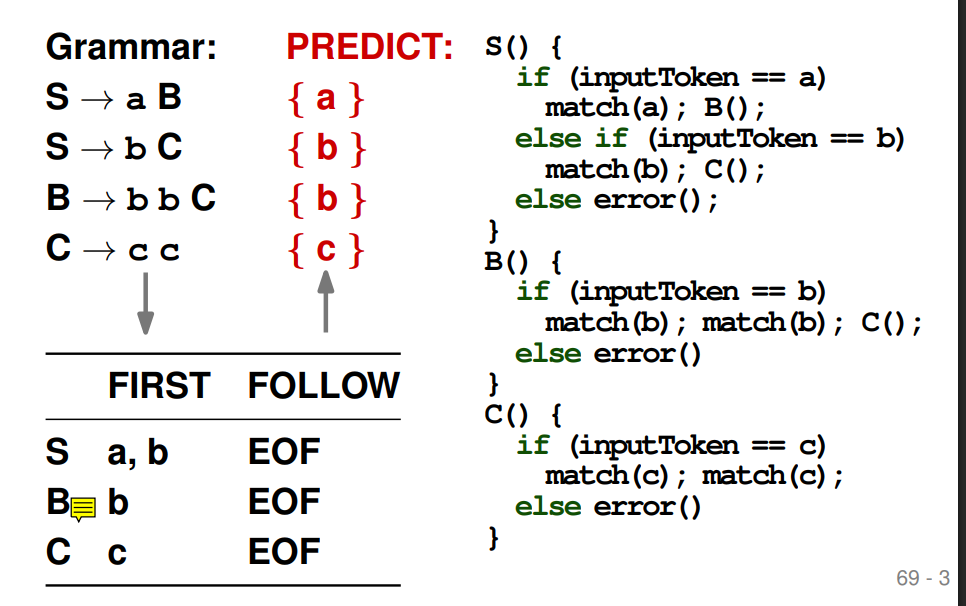
\includegraphics[scale=0.5]{assets/predict_set.png}
\end{center}

\paragraph{Computing the Parse Table (LL(1))}

\begin{itemize}
  \item Define a table $M: N \times T \to$ \{production rule, error\}
  \item For each production $A \to \alpha$:
  \begin{itemize}
    \item For each terminal $t \in \text{PREDICT}(A \to \alpha)$:
    \[
    M[A][t] = A \to \alpha
    \]
  \end{itemize}
\end{itemize}

And then for the actual parsing, we use like a stack-based approach. And for each iteration we end up looking up a table entry. If no value is found, error, and no more than one value can be found.

\subsubsection{Bottom-up Parser}
They are $LR(k)$ parsers, with Left-to-right scanning, Right-most derivation, k-tokens look ahead.

Hard to do by hand, usually done by automatically generated table.

\paragraph{Shift Reduce Algorithm} Repeat the following until all tokens read and all symbols reduced to start symbol.
\begin{lstlisting}
  Shift(read) input tokens
  Try to reduce group of symbols into single non-terminal
\end{lstlisting}

This has sometimes issues, because there can be multiple 'paths' to take.

\paragraph{Table-based LR parsing} You have two tables
\begin{itemize}
  \item Action table: $state \times T \to $reduce/shift/accept/error
  \item Goto table: $state \times N \to state$
\end{itemize}
Then also use a stack of (symbol,state) pairs to record what was seen in the past

These tables are generated using a \textbf{characteristic finite state machine}

\section{Names, Scopes, Bindings}

\subsection{Bindings}
A binding is an association between a name and an entity.  
For example, a variable name is bound to a memory location (object).

Different programming languages define different binding rules.

---

\subsection{Scopes}
\begin{itemize}
  \item \textbf{Scope of a binding:} The textual region where a specific binding is active
  \item \textbf{Scope:} The maximal region where bindings do not change
\end{itemize}

---

\subsection{Object Lifetime}
\begin{itemize}
  \item Global variables: exist for the entire program execution
  \item Local variables: exist during function execution (or scope lifetime)
\end{itemize}

\paragraph{Object Lifetime vs Binding Lifetime}
A single object can be bound multiple times.  
This means bindings can overlap or coexist, even if the object itself is the same.

---

\subsection{Storage Allocation}

Three main types of memory:

\begin{itemize}
  \item \textbf{Static:} Fixed (absolute) addresses
  \item \textbf{Stack:} Used for function calls (allocated on call, deallocated on return)
  \item \textbf{Heap:} Dynamically allocated memory at arbitrary times (slower, more flexible)
\end{itemize}

---

\subsubsection{Statically Allocated Memory}
Depends on the language, but typically used for:
\begin{itemize}
  \item Global variables
  \item Constant literals
  \item Symbol tables
  \item etc.
\end{itemize}

---

\subsubsection{Stack Memory}
Think of it as a stack of function calls.

Each function call creates a \textbf{stack frame}, which contains:
\begin{itemize}
  \item Function arguments
  \item Local variables
  \item Temporary values
  \item Return address
\end{itemize}

---

\subsubsection{Heap-Based Allocation}
Used for objects whose size is not known at compile time.

\textbf{Example:} dynamically allocated data structures.

Some programming languages use \textbf{managed memory}:
\begin{itemize}
  \item Unreachable objects are automatically deallocated (garbage collection)
  \item Easier to use, but less control and potential overhead
\end{itemize}

---

\subsection{Scoping Rules}
Scoping rules determine which bindings are active at a given point.

\subsubsection{Nested Scope}
Inner (deeper) scopes usually override outer ones.

---

\subsubsection{Static vs Dynamic Scoping}

\paragraph{Static Scoping (Lexical Scoping)}
Binding is determined by the program text.

You resolve a name by moving outward through nested scopes.

\textbf{Important:} Order inside a scope usually does not matter (a declaration below can still be used above, depending on the language).

---

\paragraph{Dynamic Scoping}
Binding depends on the \textbf{control flow} at runtime.

You resolve a name by walking up the \textbf{call stack} until a binding is found.

---

\subsubsection{Built-in Objects}
Most programming languages have built-in objects/functions:
\begin{itemize}
  \item They exist in the outermost scope
  \item Accessible from everywhere
\end{itemize}

They can often be overwritten → this is called \textbf{Monkey Patching}.

---

\subsection{Aliasing and Overloading}

\subsubsection{Aliasing}
Two or more names refer to the same memory location.

\begin{lstlisting}[language=C]
double n = 5.0;
double* p = &n;
\end{lstlisting}

---

\subsubsection{Overloading}
Multiple definitions for the same name (usually functions).

\begin{lstlisting}[language=Java]
class Overload {
  void foo() {}
  void foo(int n) {}
  void foo(String s) {}
}
\end{lstlisting}

Which function is called depends on the arguments.

---

\subsection{Referencing Environment}
The complete set of bindings visible at a specific point in a program.

This is determined by the scoping rules.

\paragraph{Example}
\begin{lstlisting}
function a() {
  var x = 23;
  function b() {
    console.log(x);
  }
  x = 42;
  return b;
}

b = a();
var x = 5;
b();
\end{lstlisting}

---

\subsubsection{Shallow Binding}
Referencing environment is created when the function is \textbf{called}.  
Used with dynamic scoping.

---

\subsubsection{Deep Binding}
Referencing environment is created when the function reference is \textbf{created}.  
Used with static scoping.

\paragraph{Closure}: Its a structure to implement deep binding. \textbf{Pointer to function code + Pointer to referencing environment}
---

\section{Control Flow}

Control flow defines the order in which instructions are executed:
\begin{itemize}
  \item Sequencing
  \item Iteration
  \item Recursion
  \item Concurrency
  \item Exceptions
\end{itemize}

---

\subsection{Expressions}

\subsubsection{Operator vs Operand}
\begin{itemize}
  \item \textbf{Operator:} Symbol/function that performs an operation (e.g. $+$, $*$)
  \item \textbf{Operand:} The values the operator acts on
\end{itemize}

---

\subsubsection{Notations}

\begin{itemize}
  \item \textbf{Prefix}
  \begin{itemize}
    \item \texttt{op a b}, \texttt{op(a,b)}, \texttt{(op a b)}
  \end{itemize}
  
  \item \textbf{Infix}
  \begin{itemize}
    \item \texttt{a op b}
  \end{itemize}
  
  \item \textbf{Postfix}
  \begin{itemize}
    \item \texttt{a b op}
  \end{itemize}
\end{itemize}

---

\subsubsection{Multiplicity}
Number of operands an operator expects:
\begin{itemize}
  \item Unary: \texttt{a++}
  \item Binary: \texttt{a + b}
  \item Ternary: \texttt{condition ? a : b}
\end{itemize}

---

\subsubsection{Order of Evaluation}
Applies to arithmetic, boolean, and pointer expressions.

Defined by:
\begin{itemize}
  \item \textbf{Precedence:} Which operators bind stronger
  \item \textbf{Associativity:} Direction of evaluation for same-precedence operators

  \textbf{Typical rules:}
  \begin{itemize}
    \item Arithmetic operators → usually left-to-right (except exponentiation)
    \item Assignment → usually right-to-left
  \end{itemize}
\end{itemize}

\begin{center}
  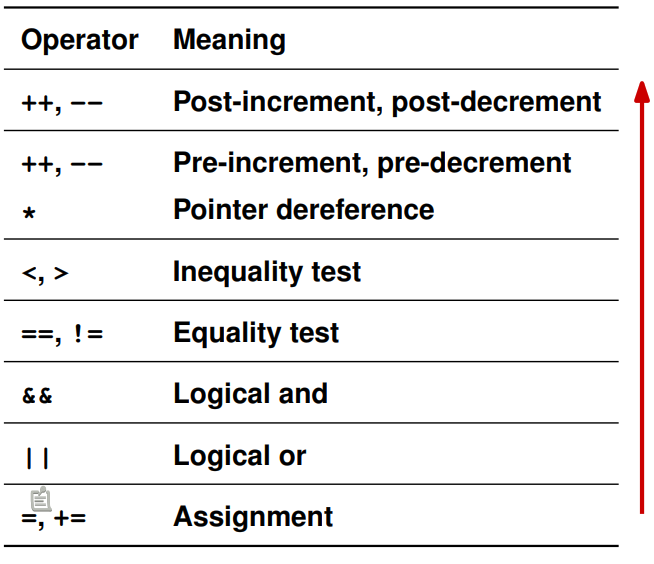
\includegraphics[scale=0.5]{assets/precedence_level_c.png}
\end{center}
\subsubsection{Ordering within expressions}
\[a - f(b) - c*d\]
Imagine $f$ alters one of the other variables. What is the orden there?

Solution: Depends on language
\begin{itemize}
  \item Java, C\#: Left-to-right
  \item C: undefined, compiler may pick the best order
\end{itemize}
\subsection{Short circuit evaluation}
Saves time when evaluating booleans.

The usual we already know $A \&\& B$, if A is false B is not computed.

Almost all PL's implement this (except notably Pascal)

\subsection{Control flow with goto statements}
Most assembly is done with conditional/unconditional jumps

Early PL's implemented goto. It jumps to statament label.

According to Djikstra, you should avoid them and use structured control flows.

\subsubsection{Continuations}
Generalization of goto's

It allows to define new control flow structures
\begin{itemize}
  \item Exceptions
  \item Iterators
  \item Coroutines
\end{itemize}

High-level definition: Context in which to continue executions

Low-level definition (three parts)
\begin{itemize}
  \item Code adress: where to continue
  \item Referencing environment
  \item Another Continuation (to be used when code returns)
\end{itemize}

Really complicated to grasp and work with, they are heavily discouraged.

\subsection{Selection}
Branch that depends on a condition (if/else, switch/case)

These are mapped to their correspondent goto statements in the compiler.

\subsection{Iteration}
There are two forms of loops
\begin{itemize}
  \item Enumeration-controlled: Once per value in finite set. Usually built with initial value, bound, step size.
  \item Logically-controlled: Repeat until boolean expression is false. The condition can be placed pre-test, mid-test or post-test
\end{itemize}
And then there are PL specific traits, like modification of variables within loop, leaving loop, skipping loop, etc.

\subsubsection{Iterators}
Special enumeration-controlled loop. Iterates through any kind of set/sequence of values. Allows to enumerate and use the individual values

Divides itself in:
\begin{itemize}
  \item True Iterators: Subrutine with $yield$ statements (each yield returns another element). Used in python for loops
  \item Iterator Objects: Regular Objects with methods for initialization, next value getter, and test for completion. Used in Java and C++
  \item First Class Functions: Divides into two functions:
  \begin{itemize}
    \item One function says what to do for each element
    \item Another function calls the first function for each element
  \end{itemize}
  Used in java streams for example
\end{itemize}
\subsection{Recursion}
Powerful construct equally as powerful as iteration. Usually less efficient than iteration, because of the stack frame overhead.

\subsubsection{Tail Recursion}
When the recursive call is the last statement before the return. The compiled code can reuse the stack frame.

\section{Type Systems}

In most programming languages, expressions and memory objects are associated with \textbf{types}. For example, the assignment $x = 4$ typically implies that $x$ belongs to a numeric type.

\subsection{Why Do We Need Types?}
Types serve several critical functions in software development:
\begin{enumerate}
    \item \textbf{Operational Context:} They define how operations are interpreted. For instance, $a + b$ might perform mathematical addition for integers but string concatenation for text.
    \item \textbf{Safety Constraints:} They prevent invalid operations, such as attempting to calculate the logarithm of a set.
    \item \textbf{Readability:} They act as documentation, making code easier to understand (though they can occasionally make code more verbose to write).
    \item \textbf{Performance:} They allow the compiler to perform specific machine-level optimizations.
\end{enumerate}

\begin{quote}
    \textbf{Note on Raw Data:} At the lowest level, bits and bytes are \textbf{untyped}. Consequently, assembly languages are generally untyped; the 'type' is only imposed by how the instructions treat the data.
\end{quote}

\subsection{Type Checking Strategies}
Type checking ensures a program adheres to its language's compatibility rules. A violation results in a \textbf{Type Error}.

\begin{lstlisting}[language=Java]
int a = 3;
String b = a - 2; // Results in a Type Error
\end{lstlisting}

\begin{itemize}
    \item \textbf{Strongly Typed:} Prevents operations on improper types. Most modern languages follow this, though C allows some exceptions (like variable-parameter functions).
    \item \textbf{Statically Typed:} Types are checked primarily at \textbf{compile-time}. While no language is 100\% static, most prioritize early error detection.
    \item \textbf{Dynamically Typed:} Type checking is deferred to the \textbf{runtime}. This is common in scripting languages like Python or JavaScript.
    \item \textbf{Gradual Typing:} A middle ground where type annotations are optional, allowing tools to check for obvious errors while maintaining flexibility.
\end{itemize}

\subsection{Polymorphism}
There are two primary ways a language handles different types through a single interface:
\begin{itemize}
    \item \textbf{Parametric Polymorphism:} Code is written generally to take a set of types as a parameter (e.g., Generics in Java: \texttt{Set<String> a;}).
    \item \textbf{Subtype Polymorphism:} A type is defined as an extension or refinement of a supertype (e.g., class inheritance).
\end{itemize}

\subsection{Special Types and Values}
\begin{itemize}
    \item \textbf{void:} Represents the absence of a type; typically has only one possible value.
    \item \textbf{null:} Indicates that a variable does not currently hold a valid value of its assigned type.
    \item \textbf{Option:} A container indicating that a value may or may not be present, helping to avoid null-related errors.
\end{itemize}

\subsection{Type Equivalence}
This determines if two types are considered 'the same.' Strategies vary across languages based on naming or memory representation.

\subsubsection{Structural Equivalence}
Types are equivalent if they share the same internal structure. 
\textbf{Issue:} It cannot distinguish between different concepts that look identical.
\begin{lstlisting}
type student = record { name: string; age: integer }
type school  = record { name: string; age: integer }
// Under structural equivalence, these are the same type.
\end{lstlisting}

\subsubsection{Name Equivalence}
Types are only equivalent if they share the same explicit name. This is used in languages like Java to ensure that distinct entities (like a Student and a School) remain separate even if their data fields are identical.

\subsection{Type Compatibility and Conversions}
\subsubsection{Type Compatibility}
Check whether combining two values is valid, regarding their types. By combining we mean
\begin{enumerate}
  \item Assignment
  \item Operators
  \item Function Calls
\end{enumerate}

Compatible types are not always equal (float vs int).

Each PL defines rules for which types are compatible

Exmaple of rules
\begin{itemize}
  \item Can assign subtype to supertype
  \item Different number types are compatible with eachother
  \item Collections of same type are compatible, even if length differs
\end{itemize}

\subsubsection{Type Conversions}
When types aren't equal they must be converted.

\begin{itemize}
  \item Cast: explicit type conversion. Programmer changes value's type from T1 to T2
  \item Coercion: implicit type conversion. PL allows value of type T1 in situations where T2 is expected
\end{itemize}

\paragraph{Runetime behavior of conversions}: There are three cases
\begin{enumerate}
  \item Types are structurally equivalent. No code generated
  \item Types have different sets of values but represented the same in memory: May need a check that the value is in target type
  \item Different low-level representations: Need special conversion instructions
\end{enumerate}


\subsubsection{Coercions in C}
Most primitive types are coerced whenever needed. Obviously, some coercions cause information loss ($float \to int$ loses fraction, $int\to char$ may cause overflow)

So the implicit conversion order is 

\[bool \to char \to short\,int \to unsigned\,int\to long\to ...\] 
\begin{center}
  (in x86 at least)
\end{center}
\subsubsection{Coercions in Javascript}
Because JS is a slop language, basically all types are coerced when needed. This is because the language sucks
\section{Formally Defined Type Systems}
Formally defined type systems provide a mathematical framework to reason about program behavior, implemented directly within a compiler to guarantee type safety before runtime.

\subsection{Typed Expressions: Syntax}
We begin by defining a simple language of booleans and numbers via the following structural grammar:
\[
t ::= \text{true} \mid \text{false} \mid \text{if } t \text{ then } t \text{ else } t \mid 0 \mid \text{succ } t \mid \text{pred } t \mid \text{iszero } t
\]

While we can intuitively guess the evaluation mechanics of these expressions, not all syntactically valid terms make semantic sense (e.g., $\text{succ false}$). We use a binary relation $t : T$ to denote that a term $t$ safely evaluates to a specific type $T$.

Our core language consists of two base types:
\begin{enumerate}
  \item $Nat$: The type representing natural numbers.
  \item $Bool$: The type representing boolean logical values.
\end{enumerate}

Type checking is governed by static inference rules. These are visually represented as fractions, where the numerator explicitly defines the \textbf{premises} (assumptions) and the denominator defines the \textbf{conclusion} (implication):

\begin{center}
  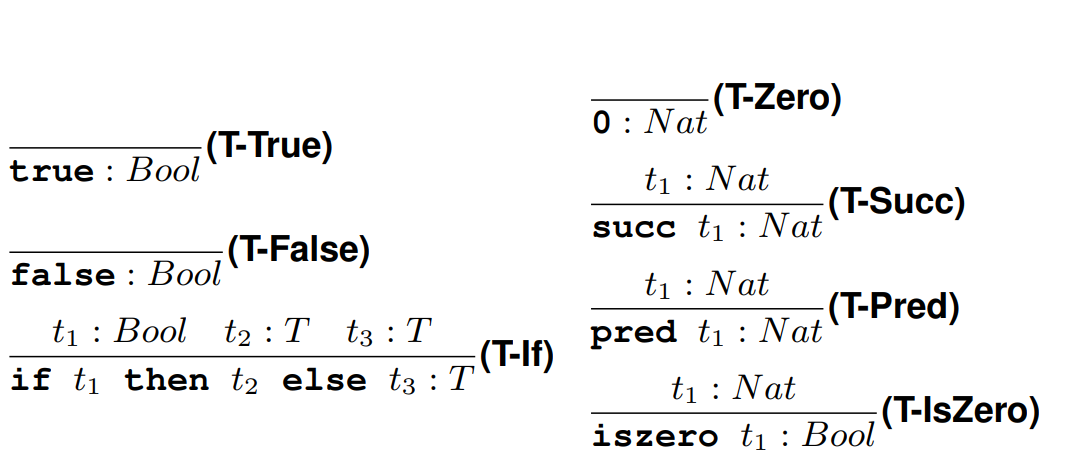
\includegraphics[scale=0.5]{assets/type_rules_1.png}
\end{center}

\paragraph{Type Checking Expressions:}
\begin{itemize}
  \item \textbf{Typing Relation:} The smallest binary relation between terms and types that satisfies all valid instances of the structural inference rules. A term $t$ is defined as \textbf{typeable} (or \textbf{well-typed}) if there exists some valid type $T$ such that $t : T$.
  \item \textbf{Type Derivation:} A structured tree composed of sequential inference rules proving that $t : T$ holds true.
\end{itemize}

\begin{quote}
\textbf{Example of a Type Derivation Tree:} 
To formally prove that the compound term $\text{iszero (succ 0)}$ is well-typed as a $Bool$, we construct a bottom-up derivation tree using our deduction rules:
\[
\frac{\displaystyle\frac{\overline{0 : Nat}}{\text{succ } 0 : Nat}}{\text{iszero (succ 0)} : Bool}
\]
Each horizontal bar represents the invocation of a typing rule, proving the target term below it is true based on the axioms above it.
\end{quote}

\subsection{The Lambda Calculus (\texorpdfstring{$\lambda$}{lambda}-Calculus)}
The $\lambda$-calculus is a foundational computational model designed to capture the structural essence of functional programming languages. It acts both as a minimal programming language and as a rigorous mathematical system.

\subsubsection{Functional Abstraction}
In pure $\lambda$-calculus, functions are first-class citizens: everything is a function. Functions accept other functions as arguments and yield functions as structural outputs.

\paragraph{Notation:} $\lambda n . \langle\text{result}\rangle$ represents an anonymous function that binds the input parameter $n$ and evaluates the body expression inside $\langle\text{result}\rangle$.

\begin{itemize}
  \item \textbf{Identity Function:} $\lambda x . x$
  \item \textbf{Negation Function:} $\lambda x . \text{if } x \text{ then false else true}$
\end{itemize}

\subsubsection{Grammar (Untyped)}
The core syntax of the untyped $\lambda$-calculus is remarkably simple, consisting of only three structural terms:
\[
t ::= x \mid \lambda x . t \mid t_1 \, t_2
\]
Where a term is either a local variable ($x$), a functional \textbf{abstraction} ($\lambda x . t$), or a function \textbf{application} ($t_1 \, t_2$). Explicit parentheses are introduced purely to remove structural ambiguity.

\paragraph{Structural Precedence Rules:}
\begin{itemize}
  \item \textbf{Left-Associativity:} Multiple function applications evaluate implicitly from left to right. Thus, the term $s \, t \, u$ is parsed precisely as $((s \, t) \, u)$.
  \item \textbf{Greedy Abstractions:} The scope body of a lambda abstraction spans as far to the right as physically possible. For example, $\lambda x . \lambda y . x \, y \, x$ evaluates as $\lambda x . (\lambda y . ((x \, y) \, x))$.
\end{itemize}

\begin{quote}
\textbf{Understanding Applications:} An application represents executing a function with a concrete argument. For example, running the expression $(\lambda x . \text{succ } x) \, 5$ substitutes the value $5$ into the variable $x$, returning $\text{succ } 5$ (which evaluates to $6$).
\end{quote}

\paragraph{Variable Scope:} An occurrence of a variable $x$ is \textbf{bound} if it falls within the body of an abstraction component $\lambda x$. If it is not enclosed by a matching abstraction, it is considered a \textbf{free variable}.

Formally, the set of free variables within a term $t$ is resolved recursively:
\[
\text{freevars}(t) = \begin{cases}
  \{x\} & \text{if } t = x \\
  \text{freevars}(t_1) \setminus \{x\} & \text{if } t = \lambda x . t_1 \\
  \text{freevars}(t_1) \cup \text{freevars}(t_2) & \text{if } t = t_1 \, t_2
\end{cases}
\]

\subsubsection{Semantics \& Evaluation}
Computation in the $\lambda$-calculus progresses step-by-step through a process called \textbf{$\beta$-reduction} (Beta-reduction). When an abstraction is applied to an argument, the parameter replaces all instances of the bound variable inside the body expression:
\[
(\lambda x . t_1) \, t_2 \to t_1[x \mapsto t_2] \quad \text{(Read: Replace all free occurrences of } x \text{ in } t_1 \text{ with } t_2\text{)}
\]
Standard deterministic computation dictates reducing the outermost, leftmost reducible expression (\textit{redex}) first.

\subsubsection{Church Encodings}
Church encodings allow us to represent standard primitives and control structures purely through function compositions.

\paragraph{Church Numerals:} Natural numbers are encoded by how many times a target function $f$ is iteratively applied to a base argument $x$:
\begin{alignat*}{3}
  0 & \;\equiv\; \lambda f . \lambda x . x \\
  1 & \;\equiv\; \lambda f . \lambda x . f \, x \\
  2 & \;\equiv\; \lambda f . \lambda x . f \, (f \, x)
\end{alignat*}

\paragraph{Church Booleans:} Booleans act as pure structural selection switches that choose between two positional parameters:
\begin{align*}
  \text{true}  & \;\equiv\; \lambda a . \lambda b . a \quad \text{(Selects the first argument)} \\
  \text{false} & \;\equiv\; \lambda a . \lambda b . b \quad \text{(Selects the second argument)}
\end{align*}

\paragraph{Conditional Branching (If-Else):} Using Church Booleans, conditional logic is written via a dedicated combinator expression:
\[
\text{if-then-else} \;\equiv\; \lambda a . \lambda b . \lambda c . a \, b \, c
\]
\begin{quote}
\textbf{Why this works:} The conditional parameter $a$ receives two inputs ($b$ and $c$). If $a$ evaluates to $\text{true}$ ($\lambda a. \lambda b. a$), it naturally yields the first option $b$. If $a$ evaluates to $\text{false}$ ($\lambda a. \lambda b. b$), it discards $b$ and outputs the second option $c$.
\end{quote}

\subsubsection{Types in Lambda Calculus}
Untyped syntax allows for meaningless expressions, such as attempting to execute a boolean variable as a function: $\text{true } \text{false}$. Because $\text{true}$ is not a function abstraction, this causes an evaluation crash. Conversely, $(\lambda x . x) \, \text{true}$ is mathematically clean.

\paragraph{Syntax of Types:}
To intercept these structural errors before execution, we formalize a set of basic types:
\[
T ::= Bool \mid T_1 \to T_2
\]
The function type constructor $\to$ is implicitly right-associative: $T_1 \to T_2 \to T_3$ parses as $T_1 \to (T_2 \to T_3)$.

\paragraph{Type Annotations:} 
To evaluate types statically, bound variables are explicitly annotated inside function abstractions:
\[
\lambda x : T_1 . t : T_1 \to T_2
\]
This states that the function accepts an input argument of type $T_1$ and evaluates to an internal body of type $T_2$.

\paragraph{Example:}
\[
\lambda x : Bool . \text{ if } x \text{ then true else false} : Bool \to Bool
\]

\subsubsection{Typing Contexts}
To properly determine types for open expressions containing free variables, we extend our simple binary typing relation ($t : T$) into a ternary relation:
\[
\Gamma \vdash t : T
\]
This reads: \textit{'Under the typing assumptions stored in the context environment $\Gamma$, the term $t$ possesses type $T$.'}

The \textbf{typing context} $\Gamma$ tracks variable-to-type map assignments for free variables. If an expression contains zero free variables (a closed term), the context is empty, which we write as:
\[
\vdash t : T
\]
\subsubsection{Typing rules}
\begin{center}
  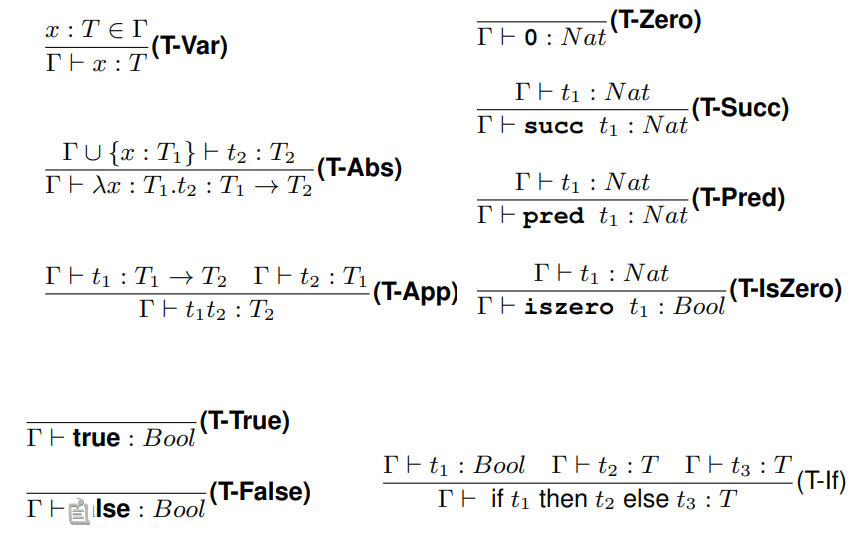
\includegraphics[scale=0.5]{assets/type_rules_2.png}
\end{center}
\section{Composite Types}
Thay are new types that are formed by joining together simpler types and using a \textbf{type constructor}

Common type constructors:
\begin{itemize}
  \item Records
  \item Arrays
  \item Strings
  \item Sets
  \item Pointers
  \item Lists
\end{itemize}

\subsection{Records}
Also called structures or \textbf{structs}

They store and manipulated related data of heterogeneous types together. Each data component is a field. First introduced in Cobol and Algol 68

Example of a struct in C
\begin{lstlisting}[language=C]
struct element{ // defines record
  char name[2]; // four fields
  int atomic_number;
  double atomic_weight;
  _Bool metallic;
}

struct element copper; // variable of record type
copper.name[0] = 'C';
// ...
if (copper.metallic) {
  // ...
}
\end{lstlisting}

\subsubsection{Variants}
Most PL's offer some type of record
\begin{enumerate}
  \item C: structs
  \item C++: Special form of class
  \item Fortran 90: Types
  \item OCaml: Tuples (order of fields is irrelevant)
  \item Java: Since Java 14 records but with immutable fields
\end{enumerate}
\subsubsection{Memory Layout}
How are they stored in memory?
\begin{itemize}
  \item Fields are usually stored in adjacent locations
  \item Field access is then Adress + Offset
  \item Alignment Constraints may create 'holes'. E.g 4-byte ints on x86 must start at address divisible by 4
\end{itemize}

\paragraph{Example: Memory layout}
\begin{lstlisting}[language=C]
struct element{
  char name[2];
  int atomic_number;
  double atomic_weight;
  _Bool metallic;
}
\end{lstlisting}

\begin{center}
  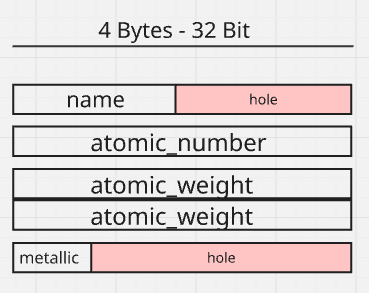
\includegraphics[scale=0.5]{assets/memory_layout_record.png}
  
  In total, 20 bytes for the entire record
\end{center}

\paragraph{Packing and Recording}
\begin{itemize}
  \item Packing: Avoid holes and break alignment. This will require additional instructions to operate on fields
  \item Reordering: Minimize holes but respect alignment.
\end{itemize}

\subsubsection{Nested Records}
Two options
\begin{enumerate}
  \item Lexically nested
  \begin{lstlisting}{language=C}
    struct outer_record{
      char some_field[10];
      struct { // no name for this inner record
        int some_other_field;
        double yet_another_field;
      } nested_field
    }
  \end{lstlisting}
  \item Fields of record type
  \begin{lstlisting}[language=C]
    struct S {
      int i;
      struct T n;
    }
  \end{lstlisting}
\end{enumerate}

\subsubsection{Reference Model vs Value Model}
Occurrence of a variable may mean a reference to its memory location or the value stored in the variable.

Java usually works by reference, C works by value.
\subsubsection{Variant Records (Unions)}
Special kind of record that reuses the same memory location for multiple variables.

It works under the assumption that variables are never used at the same time, so the size of the record is the size of the largest member.

\paragraph{Use cases}: For example, you can use it to store a pixel in different ways (RGB, YCbCr, HEX) and such. Don't need to redundantly use different variables when you can use the same one.

\subsection{Arrays}
Conceptually it's a mapping from \textbf{index type} to \textbf{element type}. Takes space in adjacent places in memory.

You can nest them into multiple dimensions. 
\subsubsection{Operations on arrays}
Not going into detail because they are known
\begin{enumerate}
  \item Slicing
  \item Comparison (element-wise) of arrays of equal length
  \item Mathematical operations
\end{enumerate}

The memory layout is continuous in memory, and varies a bit for multiple dimensions depending on the PL.

\begin{enumerate}
  \item C: Row major order. First the first row, then sequentially the second row and so on
  \item Fortran: Column Major Order. First the first column, then sequentially the second column and so on.
\end{enumerate}

The layout is essential, as it determines the efficiency of nested loops that iterate through multi-dimensional arrays. Caching can make iterating super efficient, but cache misses make everything significantly slower.

\subsection{Pointers and recursive types}
\begin{itemize}
  \item Pointer: Reference to location of memory object (an address)
  \item Recursive Type: Composite type with reference to objects at the same time 
\end{itemize}

This is strongly linked with the \textbf{reference vs value model}
\subsubsection{Operations on Pointers}
\begin{itemize}
  \item Creation: We can do it implicitly when calling a constructor, or use a built-in function that allocates heap memory and returns memory to it (malloc in C). We can also use the address-of operator (*).
  \item Allocating Memory: A pointer itself is only an adress. We need enough memory for our objects. Some PL's make it implicit, others have to be explicitly determined.
  \item Dereferencing: Access memory object refers to accesing entire object (dereferencing operator). Access fields of record that the pointer refers to (right arrow notation in C++)
  \item Deallocation: Memory must be reclaimed at some point, otherwise memory leak. Some PL's have explicit deallocation (Rust, C). If it's implicit, it's called \textbf{Garbage collection} (Java, C\#, Python)
\end{itemize}

\subsubsection{Pointers and arrays in C}
They are closely linked language constructs

This is all the same thing (the 4 last lines)
\begin{lstlisting}[language=C]
int n;
int *a;
int b[5] = {1,2,3,4,5};

a = b;
n = a[3];
n = *(a+3);
n = b[3];
n = *(b+3);
\end{lstlisting}

Array access is the same thing as pointer arithmetic

\[E1[E2] = (*((E1) + (E2)))\]
So funnily, arr[3] is the same as 3[arr]

The main difference is allocation. Arrays are implicitelly deallocated.

\subsubsection{Dangling References}
It is a live pointer that no longer points to a valid object. It is dual to memory leaks.

Happens when
\begin{enumerate}
  \item Pointer to stack object escapes it's surrounding context. (Pointers to local variables)
  \item Heap object is explicitely deallocated, but pointer lives on. (using pointer after free)
\end{enumerate}

\subsubsection{Garbage collection}
It is memory deallocation managed by the PL implementation. It avoids dangling references and such, but costs performance.

\paragraph{Reference Counts: } We use one counter for each memory object. Increment when pointer created and decrement when pointer destroyed. Deallocate when count is zero.

\paragraph{Circular dependencies: } Something like a doubly linked list have circular references, so even though the object is useless the PL may not recognize that.

So the better approach is saying that object o is useless unless there is a chain of valid pointer

\paragraph{Mark and sweep: } Algorithm to identify useless blocks

\begin{enumerate}
  \item Walk heap and mark every block as useless
  \item Start from external references (i.e names in programm) and mark every reachable block as useful
  \item Move all useless block to free list.
\end{enumerate}
\paragraph{Optimizations and other algorithms}: There are various improvements to mark and sweep:
\begin{enumerate}
  \item \textbf{Pointer reversal:} Eliminates the need for an auxiliary traversal stack during the marking phase. It temporarily reverses the heap pointers themselves to track the return path, achieving $O(1)$ space complexity.
  \item \textbf{Stop-and-copy:} Divides the heap into two halves (\textit{From-Space} and \textit{To-Space}). When one fills up, execution stops, and livepoly objects are copied compactly into the other half. This completely eliminates memory fragmentation but halves the available heap space.
  \item \textbf{Generational garbage collection:} Based on the hypothesis that 'most objects die young.' The heap is split into generations (e.g., young and old). The young generation is collected frequently and quickly; survivors are promoted to the old generation, which is scanned less often.
\end{enumerate}
\section{Control Abstraction}
\subsection{Control vs Data Abstraction}
A control abstraction abstracts a well defined operation (e.g a subroutine). A Data Abstraction abstracts how to represent information, such as types and classes.

\subsection{Terminology}
\begin{enumerate}
  \item Subroutine: Mechanism for control abstraction
  \begin{itemize}
    \item Function: Subroutine with return value
    \item Procedure: Subroutine without return value
  \end{itemize}
  \item Parameters
  \begin{itemize}
    \item Actual parameters: data passed by caller
    \item Formal parameters: data recieved by callee
  \end{itemize}
  \item Calling Sequences: It's low level code to maintain call stack. Happens four times
  \begin{enumerate}
    \item Before subroutine call inside the caller
    \item At beginning of subroutine in callee \textbf{prologue}
    \item At the end of subroutine in callee \textbf{epilogue}
    \item After subroutine inside caller
  \end{enumerate}
  They are important to understand performance / security implications
\end{enumerate}
\subsection{Reminder: Stack Layout}
Each procedure call has one stack frame made up of 
\begin{enumerate}
  \item Frame pointer: The base address used to access data in current stack frame
  \item Stack Pointer: First unused location in current stack frame
\end{enumerate}
\subsection{Call Sequence tasks}
It's tasks are the following
\begin{enumerate}
  \item Pass parameters and return values
  \item Update program counter
  \item Save return address
  \item Save and restore registers
  \item Updated stack and frame pointers
\end{enumerate}
\subsection{Typical Calling Sequence}
\begin{enumerate}
  \item Tasks done by caller before call
  \begin{itemize}
    \item Save registers whose values may be needed later
    \item Compute values of arguments and move them into stack/registers
    \item Pass return address and jump to subroutine
  \end{itemize}
  \item Tasks in prologue
  \begin{itemize}
    \item Allocate a frame
    \item Save old frame pointer on stack and update to point to the new frame
    \item Save registers from old subroutine to avoid overwriting
  \end{itemize}
  \item Steps in epilogue
  \begin{itemize}
    \item Move return value into register/stack
    \item Restore registers
    \item Restore frame and stack pointer
    \item Jump back to return address
  \end{itemize}
  \item Steps done by caller after call
  \begin{itemize}
    \item Move return value to where it is needed
    \item Restore registers
  \end{itemize}
\end{enumerate}
\subsection{Stack smashing}
It's a special kind of \textbf{buffer overflow vulnerability}. If out of bounds checks are wrong, may write beyond space allocated for local variable, allowing to rewrite e.g the return address and jump into malicious code

\subsection{Coroutines}
It's a control abstraction that allows suspending executing and resuming after suspension. Used to implement multi-tasking.

\subsubsection{Coroutines vs Threads}
Coroutines have explicit transfer of control, and only one coroutine runs at a time. 

In threads, control flow transfered implicitely and preemptively. Multiple threads may run concurrently.

\subsubsection{Coroutines vs Continuations}
In coroutines, old program counter is saved when suspending, and when resuming we continue where we left off.

In continuations, whenever jump we always start in the same position, so old programm counter is lost.

\subsection{Asynchrony}
\subsubsection{Motivation}
Parts of a programm may take very long, so we would want to continue with the rest of the programm in the meantime.

\subsubsection{Expressing Asynchrony}
\begin{itemize}
  \item Event-driven programming: Paradigm where the execution of programm is based by events, so ideal for async. The issue is mainly a deeply nested control flow, and error handling is scattered throughout the code. Sync is also tough.
  \item Promises (futures): It is an object to represent a not yet computed value. Can have one of three states
  \begin{itemize}
    \item Pending
    \item Resolved
    \item Rejected
  \end{itemize}
  Control flow easier to understand than event-driven programming. Explicit sync with Promise.all, and all error handling in one place. However, verboser syntax.
  \item Async and await: Same as futures but with some sugar to make programming with it easier. We label a function async as it performs async computation. It returns a promise, and may await other async functions. Easy error handling
\end{itemize}

\section{Data Abstraction}
The idea is to describe a class of memory objects and their associated behavior.

An abstract data type has a set of values and set of operations (e.g \textbf{Stack}, with the values being the data on the stack and the operations being push, pop, peek, etc.)

\subsection{Classes and Objects}
Classes are the most basic way of data abstraction, with encapsulation and information hiding. Objects are:
\begin{itemize}
  \item Instances of classes in class based PL's (Java)
  \item Primary entities in prototype-based PL's (JavaScript)
\end{itemize}
\subsubsection{Inheritance}
We reuse code by defining a new abstraction as extension of an existing abstraction. A subclass inherits members of superclass, and can add/modify it's members.

\paragraph{Subclasses vs Subtypes: }Are subclasses a subtype of the superclass? 

In principle, \textbf{no}.
\begin{itemize}
  \item Subclassing is reusing code inside a class
  \item Subtyping enables code reuse in clients of a class.
\end{itemize}
But in practice, most PLs merge these concepts.

\paragraph{Liskov's Substitutability Principle}: Each subtype should behave like the supertype when being used through the supertype.

\begin{itemize}
  \item Let B be subtype of A
  \item Any object of type A could be replaced with type B
  \item Any programming against A should also work with obejcts of type B
\end{itemize}

\paragraph{Modifying inherited Members: } Depends on the PL, Java allows overriding everything, C++ the elder function must be declared as \textbf{virtual}

Can a subclass hide inherited members? In Java, subclass can't \textbf{change} the visibility of members. In Eiffel, subclass can both restrict and increase visibility. 

In C++
\begin{itemize}
  \item Subclass can decrease visibility, but not increase it.
  \item Subclass can hide superclass methods by deleting them.
  \item Public/protected/private inheritance makes it so that the inherited members are \textbf{at most} public/protected/private.
\end{itemize}

\subsubsection{Initialization }
A class can have zero, one or more \textbf{constructors}. They vary by argument number and type (In Eiffel constructors can vary by name).

In some PL's (Java) constructor must be called explicitly always. In C++ it can sometimes be called implicitly (usually calls zero argument constructor).

\paragraph{Superclass constructors: } During initialization of subclass, they also initialize inherited superclass fields. Constructor of superclass is called first.

\subsubsection{Destructors}
In some PL's each class can define a destructor. It is called when the object is out of scope or the delete operand is called.

Highly recommended if the class dynamically allocates memory (where you must free the memory otherwise memory leak).

\paragraph{Execution order of destructors}: The destructor of the subclass is called before the one of the superclass. 

\subsubsection{Finalization}
Java and C\# don't have destructors but \textbf{finalizers}. They are called inmediatly before object gets garbage-collected. Used to clean up resources like file handles. 

In some short running programms it may never even be called.

\subsubsection{Dynamic Method Binding}
\paragraph{Static vs Dynamic}: If we have a subclass that defines a method already defined in the superclass. Which method gets called? (based on type of variable and type of object the variable refers to)

\paragraph{Static method binding}: Bind method based on type of variable (can be done at compile time).

\paragraph{Dynamic method binding}: Bind method based on the type of object the variable refers to. Can usually only be done at runtime. The correct method to call is found via a \textbf{Virtual method table (vtable)}. Every object points to a table with its methods

Each of them has their own pros and cons. PL's like python have dynamic binding for all methods, Java default is dynamic but you can set methods as non-overridable. C++ has static as default, but option for dynamic

In Java, 'final' keyword to dissalow overriding, and in C++, 'virtual' to allow overriding (and use dynamic binding) 
\section{Concurrency}
\subsection{Motivation}
Mixture of wanting to exploit hardware parallelism, and capturing the logical structure of a problem.

Terminology
\begin{itemize}
  \item Concurrent: Two or more running tasks whose execution
may be at some unpredictable point
  \item Parallel: Two or more tasks are actively executing at the
same time
  \item Distributed: Physically separated processors
\end{itemize}

\subsection{Levels of Parellelism}
\begin{itemize}
  \item Signals propagating through circuits
  \item Instruction-level parallelism (e.g loading from memory while another program executes)
  \item Vector parallelism: GPUs executing single instruction on a vector of data
  \item Thread-level parallelism
\end{itemize}
\subsection{Data Race}
Two accesses of the same shared memory, with at least one of them being a write, and the ordering of the accesses is non-deterministic

\subsection{Processes, Threads, Tasks}
\begin{itemize}
  \item Process: Operating system construct that can execute threads
  \item Thread: Active entity that runs concurrently with other threads (from the programmers view at least)
  \item Task: Unit of work that must be done by some thread 
\end{itemize}
\subsection{Communication}
To pass information between threads
\begin{itemize}
  \item Shared memory
  \item Message passing
\end{itemize}

\subsubsection{Thread Creation and Management}
Depends on the PL, each provides different constructs
\begin{itemize}
  \item Co-begin: Compound statement where all statements are executed concurrently
  \item Parallel loops: Loop whose iterations execute concurrently
  
  To data share here, some PL's can specify which variables are shared among the threads.
  \item Fork (with join): Fork is the explicit creation of a thread, and join is to wait a previously forked thread to terminate
  \item POSIX threads aka pthreads: It's a low-level API to create and manage threads. Very flexible, but hard to use. Supported by C and C++. 
  
  Creation
  \begin{lstlisting}[language=C]
    #include <pthread.h>

    pthread_t thread_id;
    pthread_create(&thread_id, NULL, thread_function, arg);
  \end{lstlisting}
  It has an ID, some optional attibutes, the function to execute in thread, and the arguments to pass in function

  Termination
  \begin{lstlisting}[language=C]
    pthread_exit((void *) return_value);
  \end{lstlisting}
  It is implicitly called when threads function terminates. You can also block and wait for another thread to join
  \begin{lstlisting}[language=C]
    pthread_join(thread_id, NULL);
  \end{lstlisting}
  
  \item Message passing: It avoids the usual pitfalls of shared memory. Done with two key constructs
  \begin{itemize}
    \item Independent threads: 'actors' in Java
    \item Messages exchanged between threads: 'Channels' in Go and Rust
  \end{itemize}
\end{itemize}

\paragraph{Thread Pools}: Used to separate tasks to execute from how they are executed in threads.

So the thread pool is a set of (idle) threads that can execute tasks. Reduces cost of startup and creation. Lets the pool implementation decide the scheduling of tasks

\paragraph{Spawn and Sync in Cilk}: It's an extension of C, where programmer expresses tasks and their dependencies.
\begin{itemize}
  \item spawn calls function to be executed as logically concurrent task
  \item sync joins all tasks spawned by ceiling task
\end{itemize}
The scheduler assigns tasks to processor cores through \textbf{work stealing}

\subsection{Implementing Synchronization}
We need mechanisms to control the relative order of operations on different threads. They must be explicit in shared-memory model (so that the variable being read reads the newest value stored), and implicit in the message-passing model(the sender recieves the message after it has been sent)

\subsubsection{Spinning vs Blocking}
They are two different forms of Sync
\begin{itemize}
  \item Spinning (busy-waiting): A thread re-evaluates a condition until it becomes true (because of some other thread)
  \begin{itemize}
    \item Spin locks: They provide mutual exclusion. In principle they can be implemented with only load and store operations, but super-linear time and space complexity. In practice, it is implemented using special hardware instructions. Read, modify and write a memory location as atomic.
    
    Naive:
    \begin{lstlisting}
      // Lock acquisition
      while (true):
        if (L == 0):
          L = 1
          break
      //Lock release
      L = 0
    \end{lstlisting}
    The issue is that multiple threads may enter the if- at the same time
    \item Barriers: No threads continue until all threads have reached specific point. It's based on atomic fetch-and-decrement.
    
    Initialize the shared countert to n. Decrement when thread reaches barrier. Last to arrive flips shared boolean that deactivates the barrier
  \end{itemize}
  \item Blocking: Waiting threads stop computation until some condition becomes true, then the scheduler reactivates the thread
\end{itemize}

\subsubsection{Goals}
\begin{itemize}
  \item Make some operations atomic, either all hapens or nothing. Can be done with mutually exclusive locks, so that only one thread enters a critical section at a time.
  \item Condition Synchronization: Delay some operation until some precondition holds
\end{itemize}
\subsubsection{Synchronization vs Parallelism}
Synchronization is needed to ensure the correctness of the computation, and it reduces the amount of possible parallelism

\subsubsection{Test-and-set}
Instruction that sets boolean to true, and returns if it was false before. Used in spin-locks.

Avoids contention caused by repeated writes. Spin lock implementation below
\begin{lstlisting}
  boolean L = false

  procedure acquire_lock(L) 
    while not test_and_set(L):
      while L:
        // nothing (spin)
  
  procedure release_lock(L)
    L = false
\end{lstlisting}

\subsubsection{Synchronization Constructs in PLSs}
\paragraph{Sync in Parallel Loops}: Usually the responsability as is moved to the developer, but some PL's have implicit sync through \textbf{forall} in Fortran 95. For a specific line, first all the reads are done on the LHS, then the writes

\subsubsection{Implicit Synchronization}
The compiler determines dependency between concurrently executed code fragments. Then automatically add sync if it's needed. In practice, it is extremely hard and \textbf{Auto-parallelization} is mainly an open problem.

\subsubsection{Memory Consistency}
When multiple locations are written concurrently, when do the writes become visible to other threads?

Usually, we expect \textbf{sequential consistency}
\begin{itemize}
  \item Each thread executes its instructions in it's own order
  \item Reads and writes are done inmediatly, shared memory acts like a global array
\end{itemize}
\paragraph{Relaxed Memory Models}: 
In practice, reads and writes may happen out of order. This is because ensuring sequentiality is often inefficient. Compilers can and will reorder instructions.
\paragraph{Memory Models of different PLs}: The issue is that different hardware implies different reordering behavior. PL's want to make it consistent within their own PL. So each PL defines it's own memory model
\begin{itemize}
  \item Java Memory Model: By default, writes to shared objects are not inmediatly visible to other threads. You can force visibility with explicit synchronization, marking fields as volatile, or ordering writes and reads via a synchronized block.
  \item C11 Memory Model
\end{itemize}
They can add \textbf{fences}, instructions to sync memory access
\subsection{Monitors}
They are objects with operations, internal state and condition variables.
\begin{itemize}
  \item One operation is active at any given time
  \item Calls to a busy monitor are delayed until the monitor is free.
  \item Operations can wait on a condition variable
  \item Operations can signal a condition variable, to allow others to resume
\end{itemize}

\subsubsection{Monitors in Java}
Every object can provide a monitor, \textbf{synchronized} keyword to acquire and remove locks.

\subsection{Conditional Critical Regions}
They are syntactically delimited, and represent a critical section. A condition must be true before entering the region. They are permitted to access a protected variable.

Syntax (pseudo code)
\begin{lstlisting}
  region protected_var when condition do

  end region
\end{lstlisting}
\subsection{Transactional Memory}
They achieve atomicity without locks. What they do is
\begin{enumerate}
  \item Speculatively execute the code
  \item Check for conflicts (i.e race condition)
  \item If conflict, commit the result, else roll back and attempt later.
\end{enumerate}


Implemented in Java in the Multiverse Library

\section{Functional languages}
\subsection{Functional Paradigm}
It's an alternative to imperative PLs. The output is the matematical function of input, there is no internal state, no side effects.

In practice though, there are some fuzzy boundaries. There are functional features in many imperative PL's (higher order functions) and vice versa(assignment and iteration)

\subsection{Historic origins}
\begin{itemize}
  \item Lambda Calculus
  \item Expressing computation based on abstraction into functions and function applicationº
\end{itemize}
\subsection{Features}
\begin{enumerate}
  \item Functions assigned to variables, passed as arguments or return values.
  \item Extensive Polymorphism (use function on different kind of values)
  \item List types and operators
  \item Structured function returns
  \item Constructors for structured objects
  \item Garbage collection
\end{enumerate}
\subsection{Purely Functional PLs}
The functions depend only on their parameters, no other global/local state. The order of evaluation is irrelevant.

Example: Haskell
\subsection{Non-Pure functional PLs}
They have a mix of functional features with assignments, like \textbf{Scheme}, which is a dialect of Lisp, or OCaml
\subsection{Function Application}
Represented as a pair of parenthesis. First expression is the function, remaining expressions are arguments

\[(+ 3\, \, 4) \text{ represents 3+4 = 7}\]
\subsection{Creating Functions}
Evaluating a lambda expression yields a function. First argument to lambda: Formal parameters. The remaining arguments are the body of the function

Example
\[(lambda \, (x) \, (* \,x \, x)) \quad \text{Function that squares value}\]
\subsection{Bindings}
Names are bound to values through \textbf{let}. The first argument is a list of name,value pairs, and second argument are expressions to be evaluated in order
\begin{lstlisting}
(let (  (a 3)
        (b 4)
        (square (lambda (x) (* x x)))
        (plus +))
      (sqrt (plus (square a) (square b))))
\end{lstlisting}
This yields 5.0
\subsection{Conditional expression}
Simple conditional expression with if
\begin{itemize}
  \item First argument: Condition
  \item Second/third argument: Value returned if condition true/false
\end{itemize}
We can also do multiway conditional expression with \textbf{cond}
\begin{lstlisting}
(if (< 2 3) 4 5)
\end{lstlisting}
And with cond
\begin{lstlisting}
(cond
((< 3 2) 1)
((< 4 3) 2)
(else 3))
\end{lstlisting}

\subsection{Dynamic Typing}
Types are determined and checked at runtime


\begin{lstlisting}
(if (> a 0) (+ 2 3) (+ 2 "foo"))  
\end{lstlisting}
This evaluates to $5$ if a is positive, else you get runtime type error
\subsection{Lists}
It's a \textbf{key} data structure in functional programming. It has various operations
\begin{itemize}
  \item car extracts first element
  \item cdr extracts all elements but the first
  \item cons joins a head to the rest of a list
\end{itemize}
Examples
\begin{lstlisting}
(car ' (2 3 4)) -> Yields 2
(cdr ' (2 3 4)) -> Yields (3 4)
(cons 2 ' (3 4)) -> Yields (2 3 4)
\end{lstlisting}
Note: The quote is to prevent interpretation from something like a literal

\subsection{Assignments}
We can achieve side effects via
\begin{itemize}
  \item set! for assignment to variables
  \item set-car! for assignment to head of list
  \item set-cdr! for assigning tail of list
\end{itemize}
\begin{lstlisting}
(let  ((x 2)
      (l ' (a b)))
      (set! x 3)
      (set-car! l ' (c d))
      (set-cdr! l ' (e))
      (cons x 1))

  Yields (3 (c d) e)
\end{lstlisting}
\subsection{Sequencing}
Cause interpreter to evaluate multiple expressions one after another with \textbf{begin}
\begin{lstlisting}
(let 
  ((n "there))
  (begin
    (display "hi ")
    (display n)))
\end{lstlisting}
\subsection{Iteration}
Looping through \textbf{do}
\begin{lstlisting}
((lambda n)
(do ((i 0 (+ i 1)) -> For i = 0; i += 1
    (a 0 b) -> List of triples that each specify new variable, initial value,
     and expression to compute next value 
    (b 1 (+ a b))) -> Another triple
  ((= i n) b) -> Termination condition with return value b
  (display b) -> Body of loop
  (display " "))) 5) -> Body of loop
\end{lstlisting}

\subsection{Programs as Lists}
It's the same syntax for programs and lists. They are called \textbf{S-expressions}. String of symbols with balanced parentheses

We can construct and manipulate an unevaluated program as list. Evaluation with \textbf{eval}

\begin{lstlisting}
(eval (cons ' + list( '2 '3)))
\end{lstlisting}
\subsection{Evaluation order}
There are two main strategies
\begin{enumerate}
  \item Applicative order: Evaluate arguments before passing them to function
  \item Normal order: Pass arguments unevaluated and evaluate once used
\end{enumerate}
\textbf{Scheme uses Applicative order}

Evaluation order also affects correctness. (Runtime error when evaluating an 'unused' subexpression).
\subsubsection{Lazy Evaluation}
Evaluate subexpressions on-demand, to avoid re-evaluating the same expression we memorize the result. In Haskell, that has no side effects, it's transparent to programmer. In PL's with side effects (Scheme), Programmer can explicitly ask for lazy evaluation.


\end{document} 







